%citations to Mastering Ethereum, ethereum blog, whitepaper and yellow paper
%ethereum made easy ICOs and enabled many scammers
%Ethereum goals 
%https://media.consensys.net/exploring-the-ethereum-2-0-design-goals-fd2d901b4c01 
%check vitalik's slides too on iphone
% Decentralization, Resilience, Security, Simplicity, Longetivity
% Main advantages of blockchain
% check vitalik's screenshots
\section{Ethereum}
In this section, we elaborate on how Ethereum expanded on Bitcoin by offering a platform for developers to build their decentralized solutions. We use the term ``decentralized" to describe the distribution of the authority and power on a system. 

In this section, we offer a brief summary of Ethereum, how it expanded on Bitcoin's idea and its purpose. 

\subsection{EVM and Turing Completeness}
Ethereum has a virtual machine for the execution of smart contracts and transactions, called \acrfull{evm}. It can be perceived as a global single threaded CPU, where every smart contract computation and transaction is executed on each node in the network. Every node in the network uses the \acrshort{evm} to ensure redundantly correct execution and consensus to agree on the answer. The \acrshort{evm}, has the capacity to be a quasi-Turing-complete state machine; ``quasi" because all execution is regulated through gas expenditure, which dictates how much computing power can be spent on a transaction. Hence, the halting problem\footnote{The halting problem refers, given input, whether a program will finish running or continue to run forever.} is solved. The behavior of the \acrshort{evm} depends on the programming language used for the smart contract. Ethereum has its own programming languages, Solidity which offers Turing completeness and Vyper which forbids certain operations to enhance security.

\subsection{Smart Contracts and Gas}
 Smart contracts are programs that live on the blockchain and are immutable, after deployment there is no turning back, no modifying or deleting\footnote{Deleting is available but has to be programmed before deployment, transaction history will remain intact after deleting}.  The smart contracts provide an API callable by anyone and the costs for each call are dictated by the smart contract computations. These costs enacted to:
 \begin{itemize}
     \item mitigate \acrshort{ddos} attacks on the network and
     \item make smart contracts efficient on computations and storage, thus incentivizing developers to optimize their solutions.
 \end{itemize}
The cost is enforced by gas, and gas is bought with wei, the minimum unit of Ethereum $1 wei = 10^{-9}ETH$. Its price is driven by the demand of the network and by the market \cite{gasstation}.
Gas and the price of ETH are decoupled, since units of gas align with computation units having a natural cost, while the price of ETH fluctuates as a result of market forces. Each operation offered by Ethereum's programming language has a specific gas price as seen here \cite{eth-ops-gas}. Fundamentally, gas is the execution fee that senders of transactions need to pay for every operation made on Ethereum. 

\subsection{Accounts and Transactions}
Ethereum has two types of accounts, contract and \acrfull{eoa}. Contracts have addresses, derived from the creator's address, but they do not have a private key - they are controlled by the logic of their smart contract code. On the other hand, \acrshort{eoa} do have a corresponding private key and as a result access to funds and contracts. Every action on the Ethereum blockchain, like Bitcoin, is carried out by transactions. Transactions are the inputs to the \acrshort{evm} to evaluate contracts, update balances and fundamentally update the state of the Ethereum.

Unlike Bitcoin, each transaction is an independent entity and accounts hold a balance, instead of tracking \acrshort{utxo}s. Substantially, a global state, as seen in figure \ref{fig:eth-world-state}, stores a list of accounts with balances, code, internal storage and the nonce\footnote{The nonce is a sequence number used to prevent message replay}. A transaction is considered valid if the account initiating the transaction has enough balance to pay for it. Finally, if the receiving account is a smart contract, it causes its code to run and as a result internal storage might be changed and more messages might be initiated.
\begin{figure}[H]
    \centering
    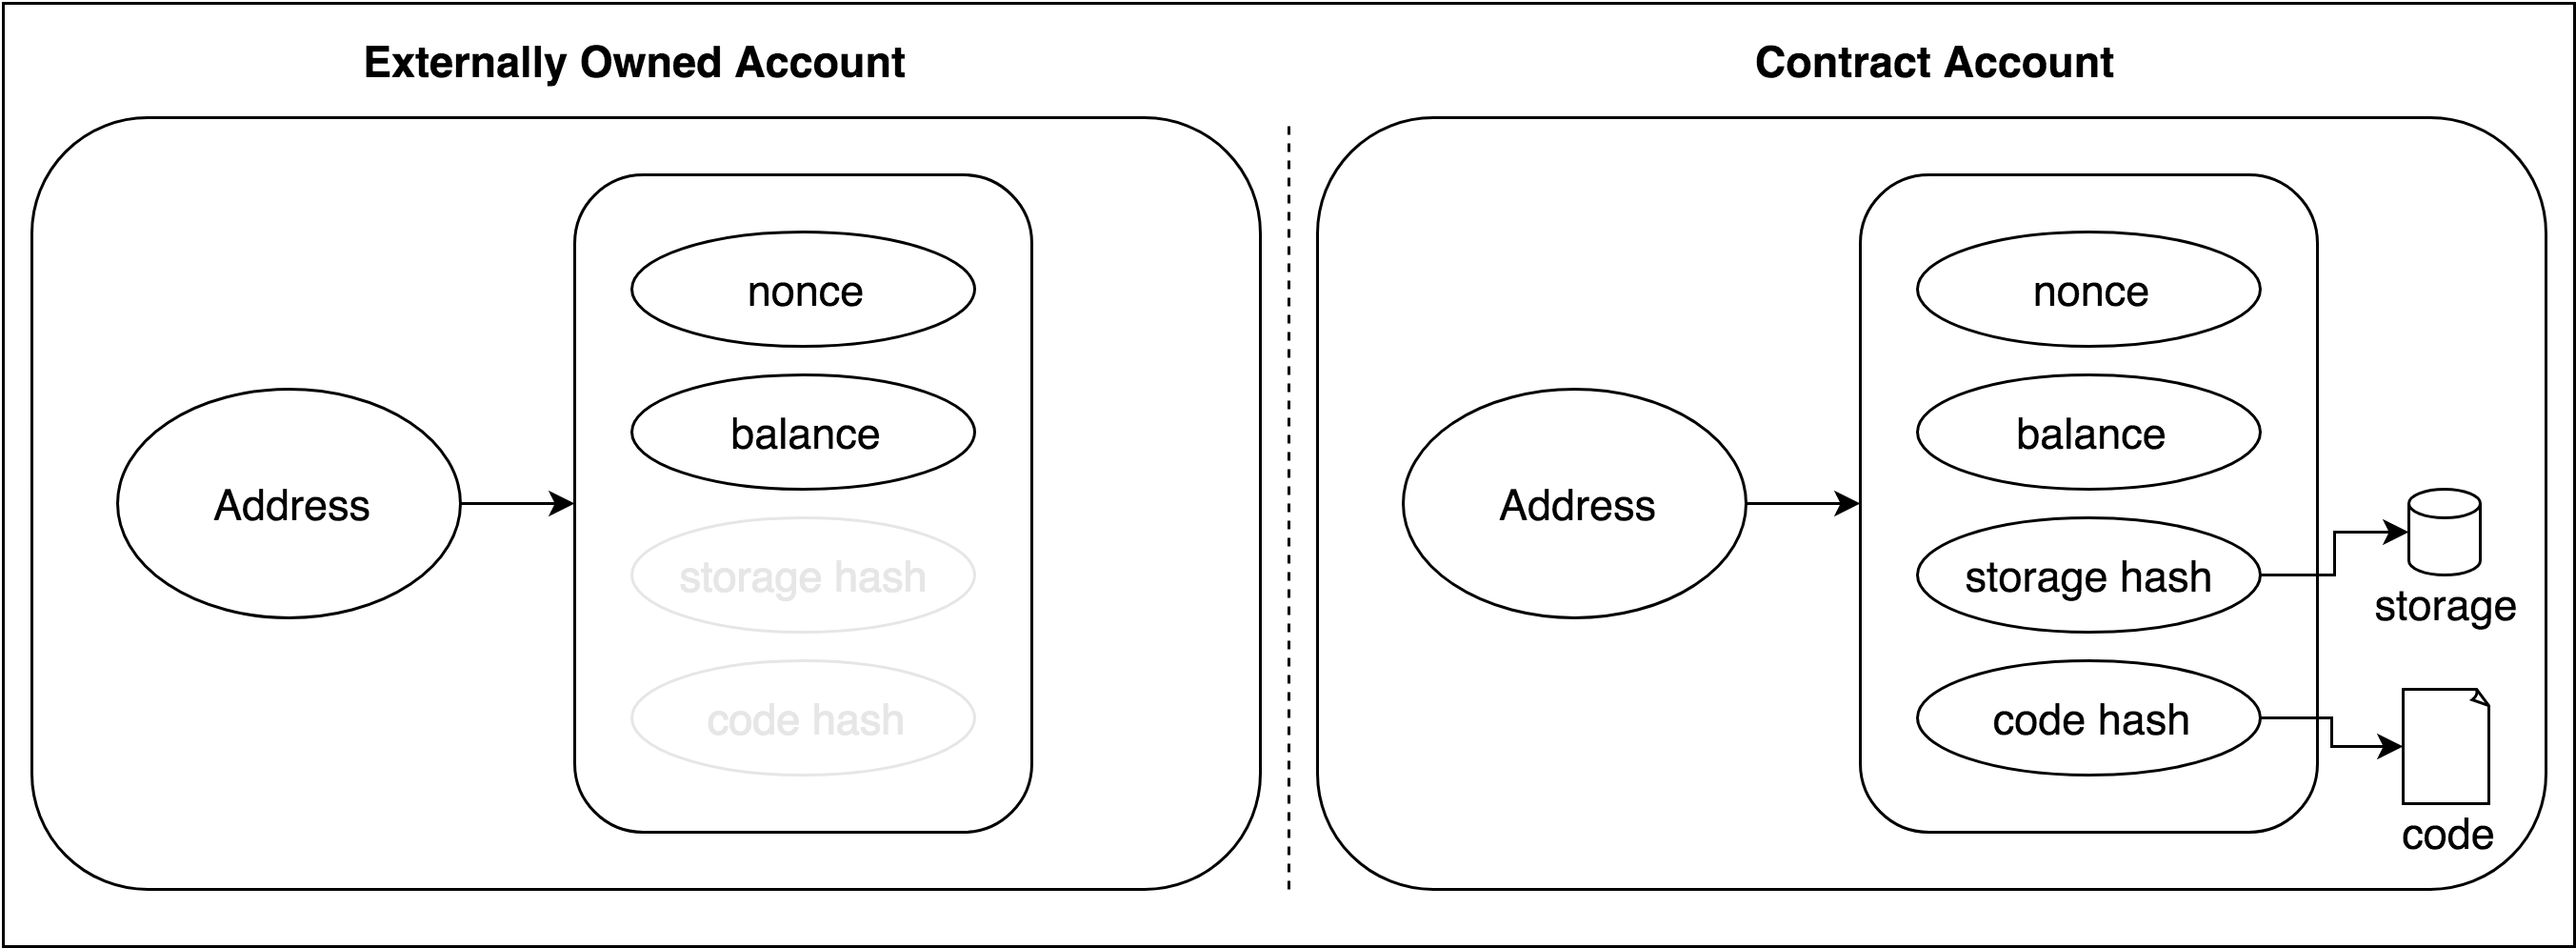
\includegraphics[width=1\textwidth]{images/world-state.png}
    \caption{Ethereum World State \cite{eth-illustrated}.}
    \label{fig:eth-world-state}
\end{figure}